\begin{frame}{Déjà trois printemps et deux hivers
(bientôt trois ?)}

\centering
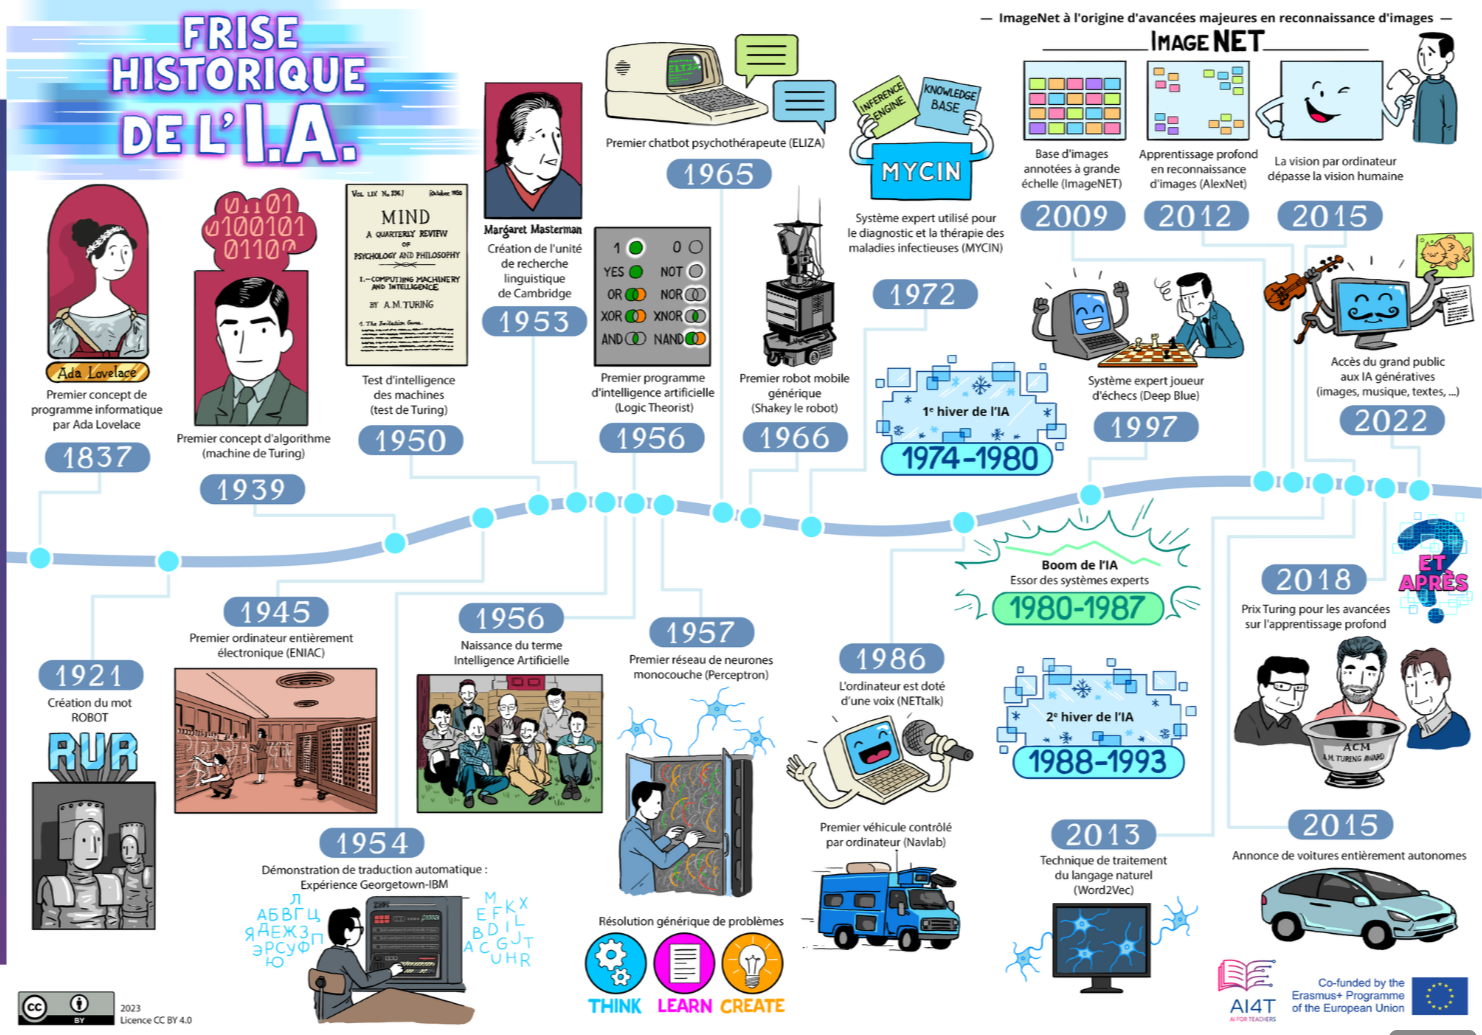
\includegraphics[width=9cm]{04_Axe1_IAG/Images/frise_ia_genially.png}
\end{frame}

\begin{frame}{Première vague : les années 1950 et les développements de l'informatique}
\textbf{Alan Turing}\\ 
\vspace{5mm}
\begin{columns}[T,onlytextwidth]
\column{0.50\linewidth}
\small
\textrightarrow{} Père de l'informatique.\\
\textrightarrow{} Article fondateur publié en 1936 qui pose les bases du binaire.\\
Rappel : Turing n'a quasiment joué aucun rôle dans la construction effective des ordi.\\ 
\textbf{Machine de Turing =} un automate imaginaire muni d’un programme et pouvant lire et écrire des caractères sur un ruban de longueur illimitée.

\column{0.60\linewidth}
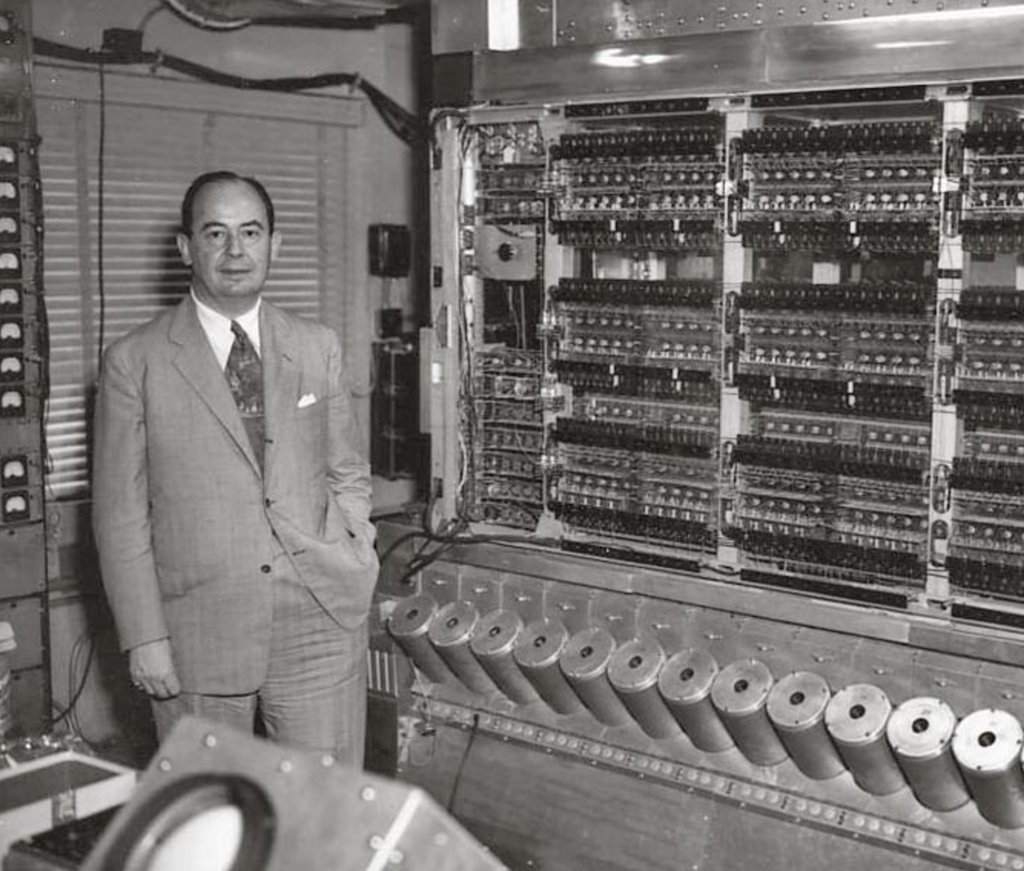
\includegraphics[width=0.80\textwidth]{04_Axe1_IAG/Images/turing.jpg}
\end{columns}

\end{frame}

\begin{frame}{Première vague : les années 1950 et les développements de
l’informatique}

\textbf{Le test de Turing (1950) : une définition de l'intelligence au miroir de la machine}

\begin{columns}[T,onlytextwidth]
\column{0.40\linewidth}
\small
\begin{itemize}
    \item "\textit{Computing Machinery and Intelligence}" (Mind, 1950)
    \item Si on intéragit avec une machine 5 minutes sans réaliser qu'on est face à une machine, alors cette machine peut être qualifiée d'"intelligente"
\end{itemize}
\column{0.50\linewidth}
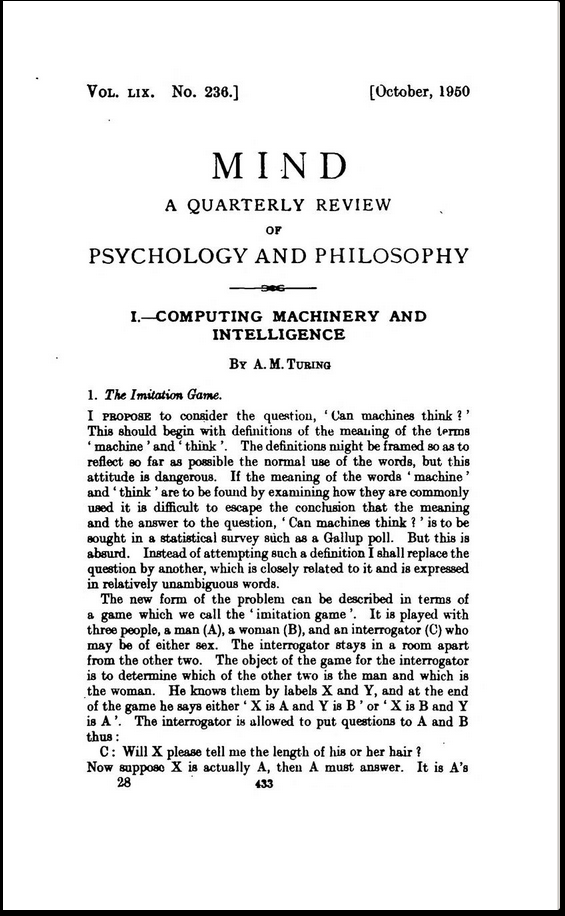
\includegraphics[width=0.50\textwidth]{04_Axe1_IAG/Images/Turing_intelligence.png}
\end{columns}
\end{frame}

\begin{frame}{Première vague : les années 1950 et les développements de
l’informatique}
\textbf{La conférence de Dartmouth et la proposition de John McCarthy (1956)}\\
\vspace{10mm}
\begin{columns}[T,onlytextwidth]
\column{0.40\linewidth}
\small
= Atelier scientifique organisé durant l'été 1956\\
= Considéré comme l'acte de naissance de l'intelligence artificielle en tant que domaine de recherche autonome\\
\textrightarrow{} Invention du terme \textit{Intelligence artificielle} par John McCarthy.
\column{0.50\linewidth}
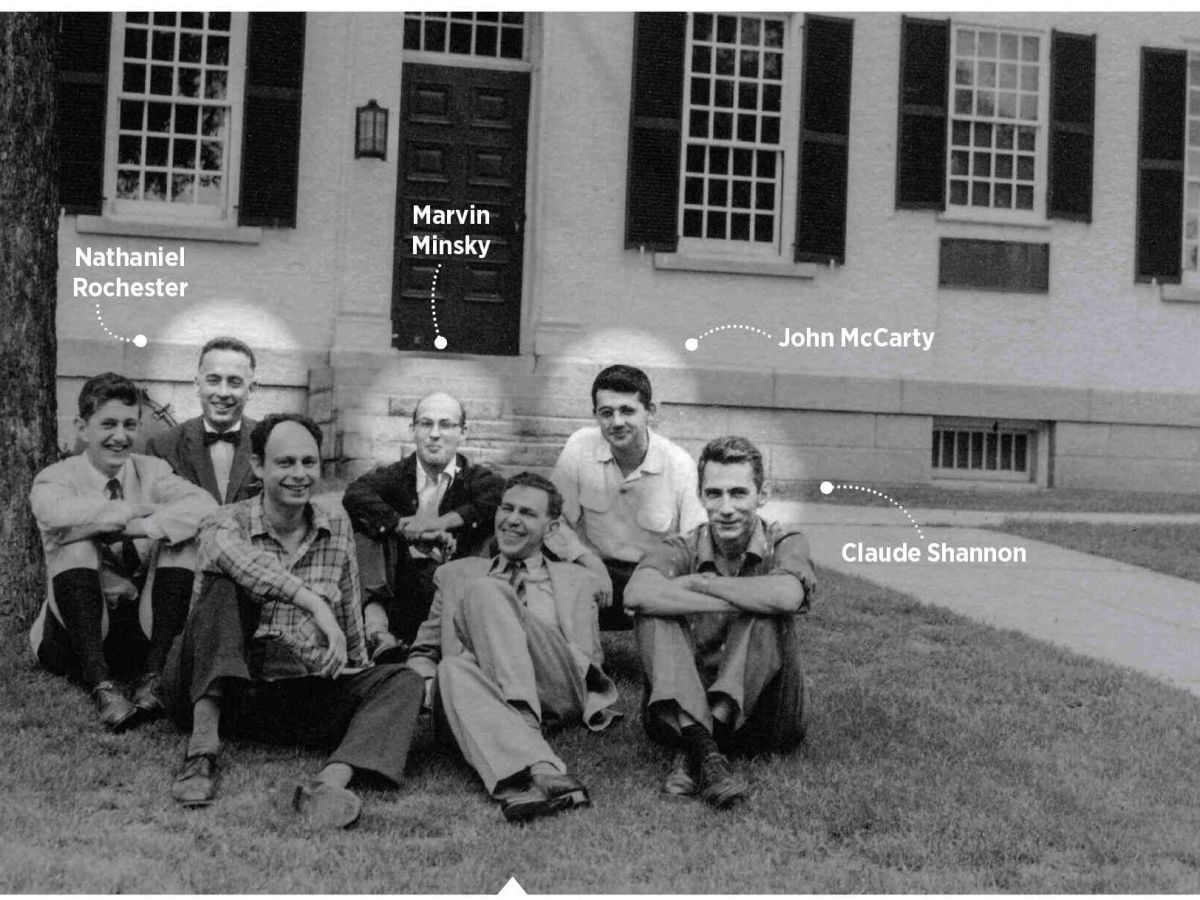
\includegraphics[width=0.90\textwidth]{04_Axe1_IAG/Images/darthmouth.jpg}
\end{columns}

\end{frame}

\begin{frame}{Seconde vague : les années 1980 et le développement des "systèmes experts"}

\textbf{Système expert }= programme informatique conçu pour simuler le savoir-faire d’un spécialiste, dans un domaine précis et bien délimité, grâce à l’exploitation d’un certain nombre de connaissances fournies explicitement par des experts du domaine.\\
\vspace{10mm}
\textbf{Exemple de système expert les plus médiatisés} : Garry Kasparov vs Deep Blue.\\
\url{https://www.youtube.com/watch?v=ZIcZymAzifM}

\end{frame}

\begin{frame}{Approche symbolique}
\centering
Les premières conceptions de l'IA s'emploient à programmer la machine pour qu'elle puisse reproduire les formes symboliques et logiques du raisonnement dit naturel. La notion d'"intelligence" est alors elle-même située : il s'agit de transférer à la machine une capacité à raisonner calquée sur le modèle humain.

Mais savons-nous vraiment comment nous pensons ?
    
\end{frame}

\begin{frame}{Seconde vague : les années 1980 et le développement des "systèmes experts"}
\centering
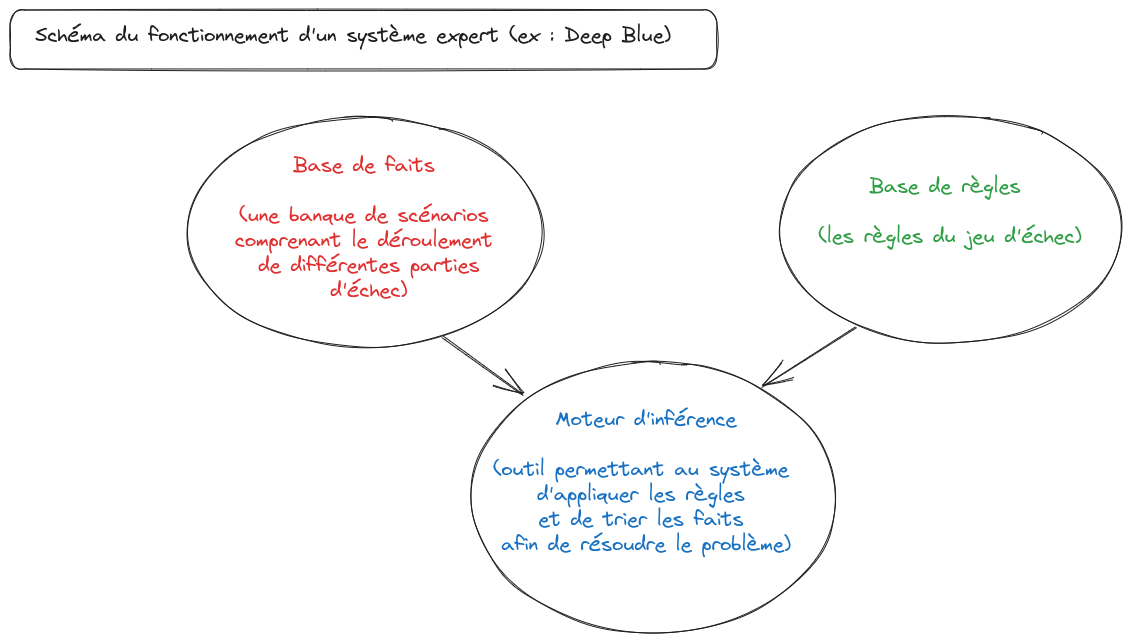
\includegraphics[width=10cm]{04_Axe1_IAG/Images/ModeleExpertSchema.png}
    
\end{frame}

\begin{frame}{Seconde vague : les années 1980 et le développement des "systèmes experts"}

\url{https://www.youtube.com/watch?v=jpCa9D2KPXM}

\begin{block}{}
    \centering
    {\small
    \textit{La réaction de Garry Kasparov immédiatement après ce match est intéressante. Il accuse l’équipe de Deep Blue d’avoir triché, d’avoir fait appel à un joueur humain pour le battre. Pour le champion du monde, aucune machine n’aurait pu à la fois jouer l’excellent 36e coup et commettre cette erreur grossière au 44e. C’est donc forcément un joueur humain qui a dicté ce coup à Deep Blue. Comme beaucoup de non-spécialistes, Kasparov ne croit pas que la machine puisse être à ce point faillible. Il est à mille lieues de la vérité.}}\\
    \textbf{Nicolas Sabouret, \textit{"Pourquoi l’intelligence artificielle se trompe tout le temps"}, The Conversation, 2020.}
\end{block}
\end{frame}

\begin{frame}{La théorie de la complexité et l'approche heuristique}
\textbf{Théorie de la complexité=} étudie formellement le temps de calcul, l'espace mémoire (et plus marginalement la taille d'un circuit, le nombre de processeurs, l'énergie consommée…) requis par un algorithme pour résoudre un problème algorithmique.\\
\vspace{3mm}
\textbf{Exemple des échecs:}
\begin{itemize}
    \item Regarder toutes les parties possibles.
    \item Le mathématicien Claude Shannon a estimé qu’il y a environ 10 puissance 120 parties d’échecs possibles.
    \item Même avec des machines avec des puissances de calcul qui doublerait tous les 2 ans (loi de Moore), impossible d'énumérer toutes ces parties!
\end{itemize}

En résumé: calculer la probabilité de tous les coups possibles est trop complexe.
\end{frame}

\begin{frame}{La théorie de la complexité et l'approche heuristique}
    \centering
    {\small
    \textit{
    Le principe des programmes d’IA est donc de calculer des solutions pas trop mauvaises à des problèmes dont on sait, mathématiquement, qu’ils ne peuvent pas être résolus de façon exacte dans un temps de calcul raisonnable. Et pour cela, il faut accepter de faire parfois des erreurs. De ne pas avoir toujours la meilleure réponse, ou une réponse complètement correcte. C’est pourquoi tout programme d’IA fait forcément des erreurs. C’est inévitable et c’est même ce qui les caractérise.}
    }\\
\textbf{Nicolas Sabouret, \textit{"Pourquoi l’intelligence artificielle se trompe tout le temps"}, The Conversation, 2020}
\end{frame}

\begin{frame}{Limite des systèmes experts, ou le second hiver de l'IA}
\begin{itemize}
    \item Coût de développement trop élevées
    \item Cantonnés à certains domaines industriels: système de signalisation des trains, système de guidage des avions...
\end{itemize}

\centering
{\small
\textit{Qu’est-ce qui n’allait pas dans l’idée d’une machine raisonnant logiquement ? Tout simplement, que le fonctionnement de la pensée humaine est impossible à reproduire. Nous prenons très rarement des décisions à partir de règles de raisonnement que nous saurions expliciter. Nos jugements sont aussi faits d’émotions, d’éléments irrationnels, de spécifications liées au contexte et de toute une série de facteurs implicites ; bref, la décision ne se laisse pas capturer par des règles formalisables.}
}\\
\textbf{Dominique Cardon, Culture numérique, Presses de Science Po, 2019}

\end{frame}

\begin{frame}{Troisième vague : le modèle connexionniste des années 2020}

\begin{block}{}
 \centering
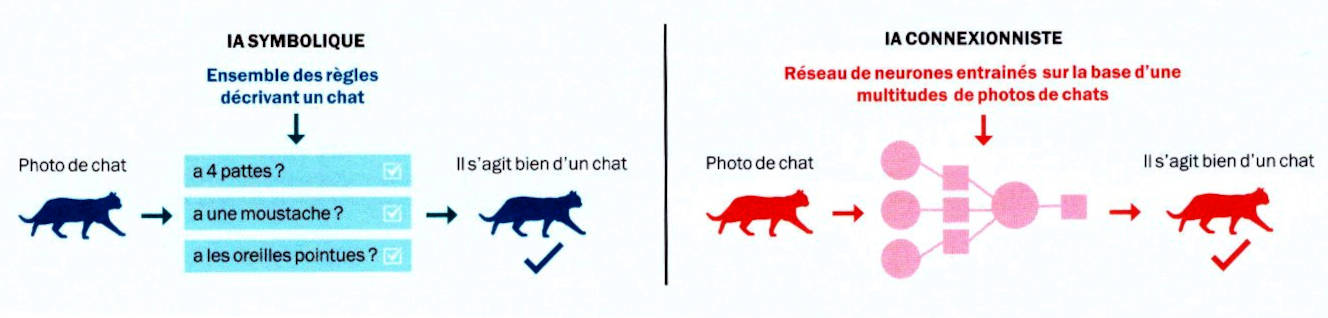
\includegraphics[width=0.90\textwidth]{04_Axe1_IAG/Images/ia-symboliqueVSconnexionniste.jpg}   
\end{block}

Luc Julia dans son ouvrage \textit{L’intelligence artificielle n’existe pas} paru en 2019 aux Éditions First
\begin{itemize}
    \item Ce n’est pas l’intelligence qui caractérise les systèmes d’IA d’aujourd’hui, mais leur capacité de \textbf{reconnaissance grâce à l’apprentissage machine}.
    \item Approche dite "connexionniste", inspirée de \textbf{la structure et du fonctionnement des réseaux de neurones biologiques}.
\end{itemize}

\end{frame}

\begin{frame}{Un concept: les réseaux de neurones}
\begin{columns}[T,onlytextwidth]
\column{0.40\linewidth}
\small
\begin{itemize}
        \item \textbf{\textit{Machine learning}}: Apprentissage à partir de réseaux de neurones artificiels, tente de reproduire le raisonnement humain.
        \item \textbf{\textit{Deep learning}}: Apprentissage à partir de réseaux de neurone profonds pour identifier des structures dans des volumes considérables de données.
    \end{itemize}
\column{0.50\linewidth}
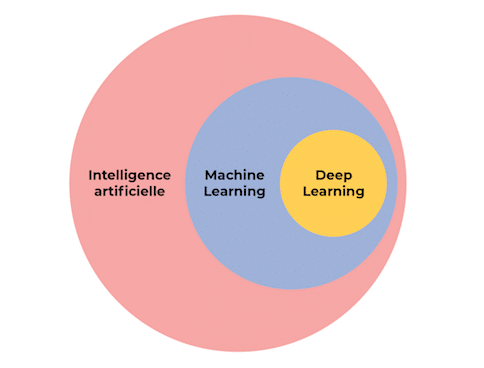
\includegraphics[width=0.80\textwidth]{04_Axe1_IAG/Images/schema_machinelearning_deeplearning.png}
\end{columns}

\end{frame}
\begin{frame}{Un concept: les réseaux de neurones}
\centering
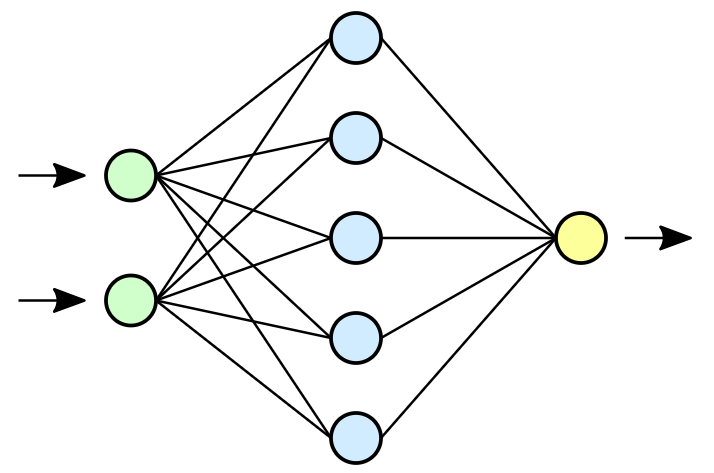
\includegraphics[width=0.60\textwidth]{04_Axe1_IAG/Images/nauronal_network.png}\\
\begin{block}{}
    \textbf{Le modèle connexionniste provoque un changement de paradigme, en nous faisant passer d'une approche modélisante à une approche statistique et probabiliste (fondées sur des modèles malgré tout : les LLM)}
\end{block}
\end{frame}

\begin{frame}{La vectorisation : vers une modélisation spatiale des termes (vs sens)}
    \textbf{Vectorisation=} Convertir des données textuelles (mots, phrases ou documents) en vecteurs numériques.\\

\begin{block}{}
    \centering
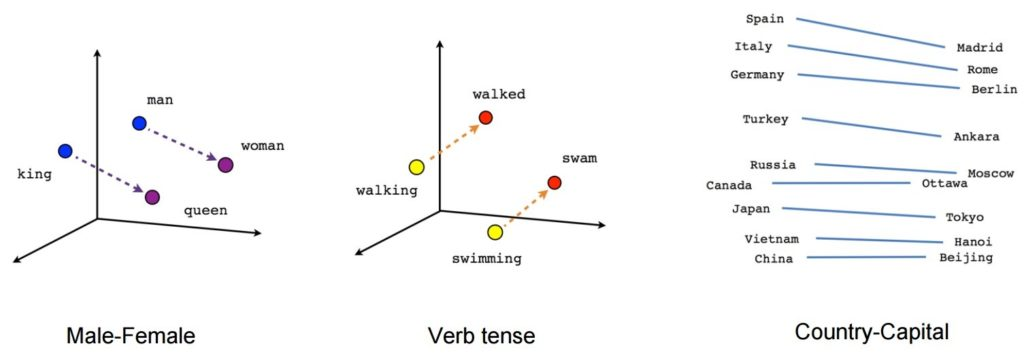
\includegraphics[width=0.70\textwidth]{04_Axe1_IAG/Images/wordvectors.jpeg}
\end{block}


\textrightarrow{}Plus les mots sont proches, plus ils ont des chances d'avoir des significations similaires, ou de s'inscrire dans un même contexte sémantique (une même relation contextuelle).

\end{frame}

\begin{frame}{La vectorisation : vers une modélisation spatiale des termes (vs sens)}
\centering
    En conséquence, lorsque vous utilisez une IAG, vous lui posez une question ou vous lui donnez une instruction en vous inscrivant dans un régime de signification. La réponse de l'IAG, en revanche, s'appuiera sur des probabilités, soit sur un calcul de proximité entre des objets vectorisés.
\end{frame}

\begin{frame}{Pour résumer}
    \textbf{Comment aimez-vous apprendre ?}\\
    \begin{itemize}
        \item \textbf{Approche symbolique} : vous préférez que l'on vous donne des consignes précises, après avoir suivi un cours magistral en amont vous présentant des règles de composition d'une dissertation, que vous allez ensuite vous-même appliquer.
        \item \textbf{Approche connexionniste} : vous préférez lire plusieurs exemples de dissertations, en tâchant de comprendre vous-mêmes comment elles fonctionnent pour les imiter.
    \end{itemize}

\end{frame}